\section{Results} 
To make the simulation easy to understand we started with the baseline model with two covariates that was split into the different model sets. We then started adding the different flexibilities one at a time to see how much each flexibility by itself would add to the FPP and FPR compared to the baseline model. Figure 1 shows the FPP and FPR for the baseline model with different data structures whereas the remaining figures in the result section can be seen as added effect regarding the different flexibilities. 
\subsection{Worst case scenario}
Under different conditions, the FPP was as high as 99\%. There were several ways to obtain a result like this. In general, the covariates needed to be binary and dummy coded and interactions used without including main effects. In such case, a 99\% FPP could be obtained with only two covariates and a big enough sample (see Figure 4). Alternatively, a 99\% FPP could also be obtained using a smaller sample and more than two covariates (see Figure 3). In the same sets, the FPR was as high as 35\%. In other words, in the sets where there was a 99\% chance to find a significant result, around 35\% of the models had either a significant main effect or interaction effect with the variable of interest. 

\subsection{Effect of model specification}
The FPP and FPR for the different model sets can be found in Figure 1. Looking at the FPP and FPR between the different sets, it is clear that the highest FPP and FPR could be obtained in the sets HCI and ME+ HCI. This was the case both when the main effects were present or not. When the main effects were not present, and the covariates and variable of interest were binary with dummy coding, the high FPP and FPR occurred because the interaction was only splitting the sample, and the true effect from the covariate was captured in the interaction. The FPP for a sample of 200 was 83.4\% for the HCI set and 86.9\% for the ME+ HCI set. When the variables were continuous and everything else equal, the FPP for the two sets was 18.9\% and 24.3\%, respectively. When we implemented the restriction that main effects should follow interactions, only the ME+ HCI set remained because the HCI set became an empty set. In that case, the FPP was 20.6\% for binary variables and 18.6\% for continuous variables. Across all sets the FPP for using two binary variables was 87.2\%, and for continuous, it was 24.7\% when we had no restrictions regarding the main effect and 22\% and 18.5\% respectively when we had such a restriction. 
Not only was the FPP high, but the FPR was also higher in some sets (see red bars in Figure 1). In general, the proportion of these models was around the expected 5\%, but in sets where there were interactions between the variable of interest and main effect was not present (left hand side of Figure 1), the FPR was above the 5\%. The percent of models with a significant variable of interest or interaction with the variable of interest was 31.9\% for the ME+ HCI set when main effects were not included and binary data was used. One way to remedy this was by coding the binary variables using effects coding. Here, the FPP fell to 20.6\%, and FPR in the ME+ HCI set dropped to 9.7\%, the same level as if the covariates were continuous (see Figure SI1 A in Supplementary information). Overall, the sets where HCI was included had a higher number of models with a significant effect. 
Adding one more covariate (such that the analysis included three) to the analysis just increased the FPP across all model sets, where it was still possible to get a higher FPP. This added effect of using one more covariate can be seen in Figure 2. The increase was the highest for the binary data and where there was no restriction that the main effect should follow the interaction. Several of the sets here had the rate of FPP just below a 100\%. This increase was also seen when we restrict the sets such that the main effects should always be present. Here the increase of adding one more covariate was 14.3\% to the FPP for the set ME+ HCI + CCI with binary data and 13.1\% for continuous data in the same set. The rates of FPR also increased. This increase, however, only applies for the sets where there were interactions between the variable of interest and the covariates. Even though there was a higher increase when there was no restriction that the main effect should be present, we observed a increase even when the restriction was present. Using three covariates increased the FPR for ME+ HCI + CCI for around 3\% compared to using two covariates with both binary and continuous data. 

% plot of main analysis
\begin{figure}[hbt!]
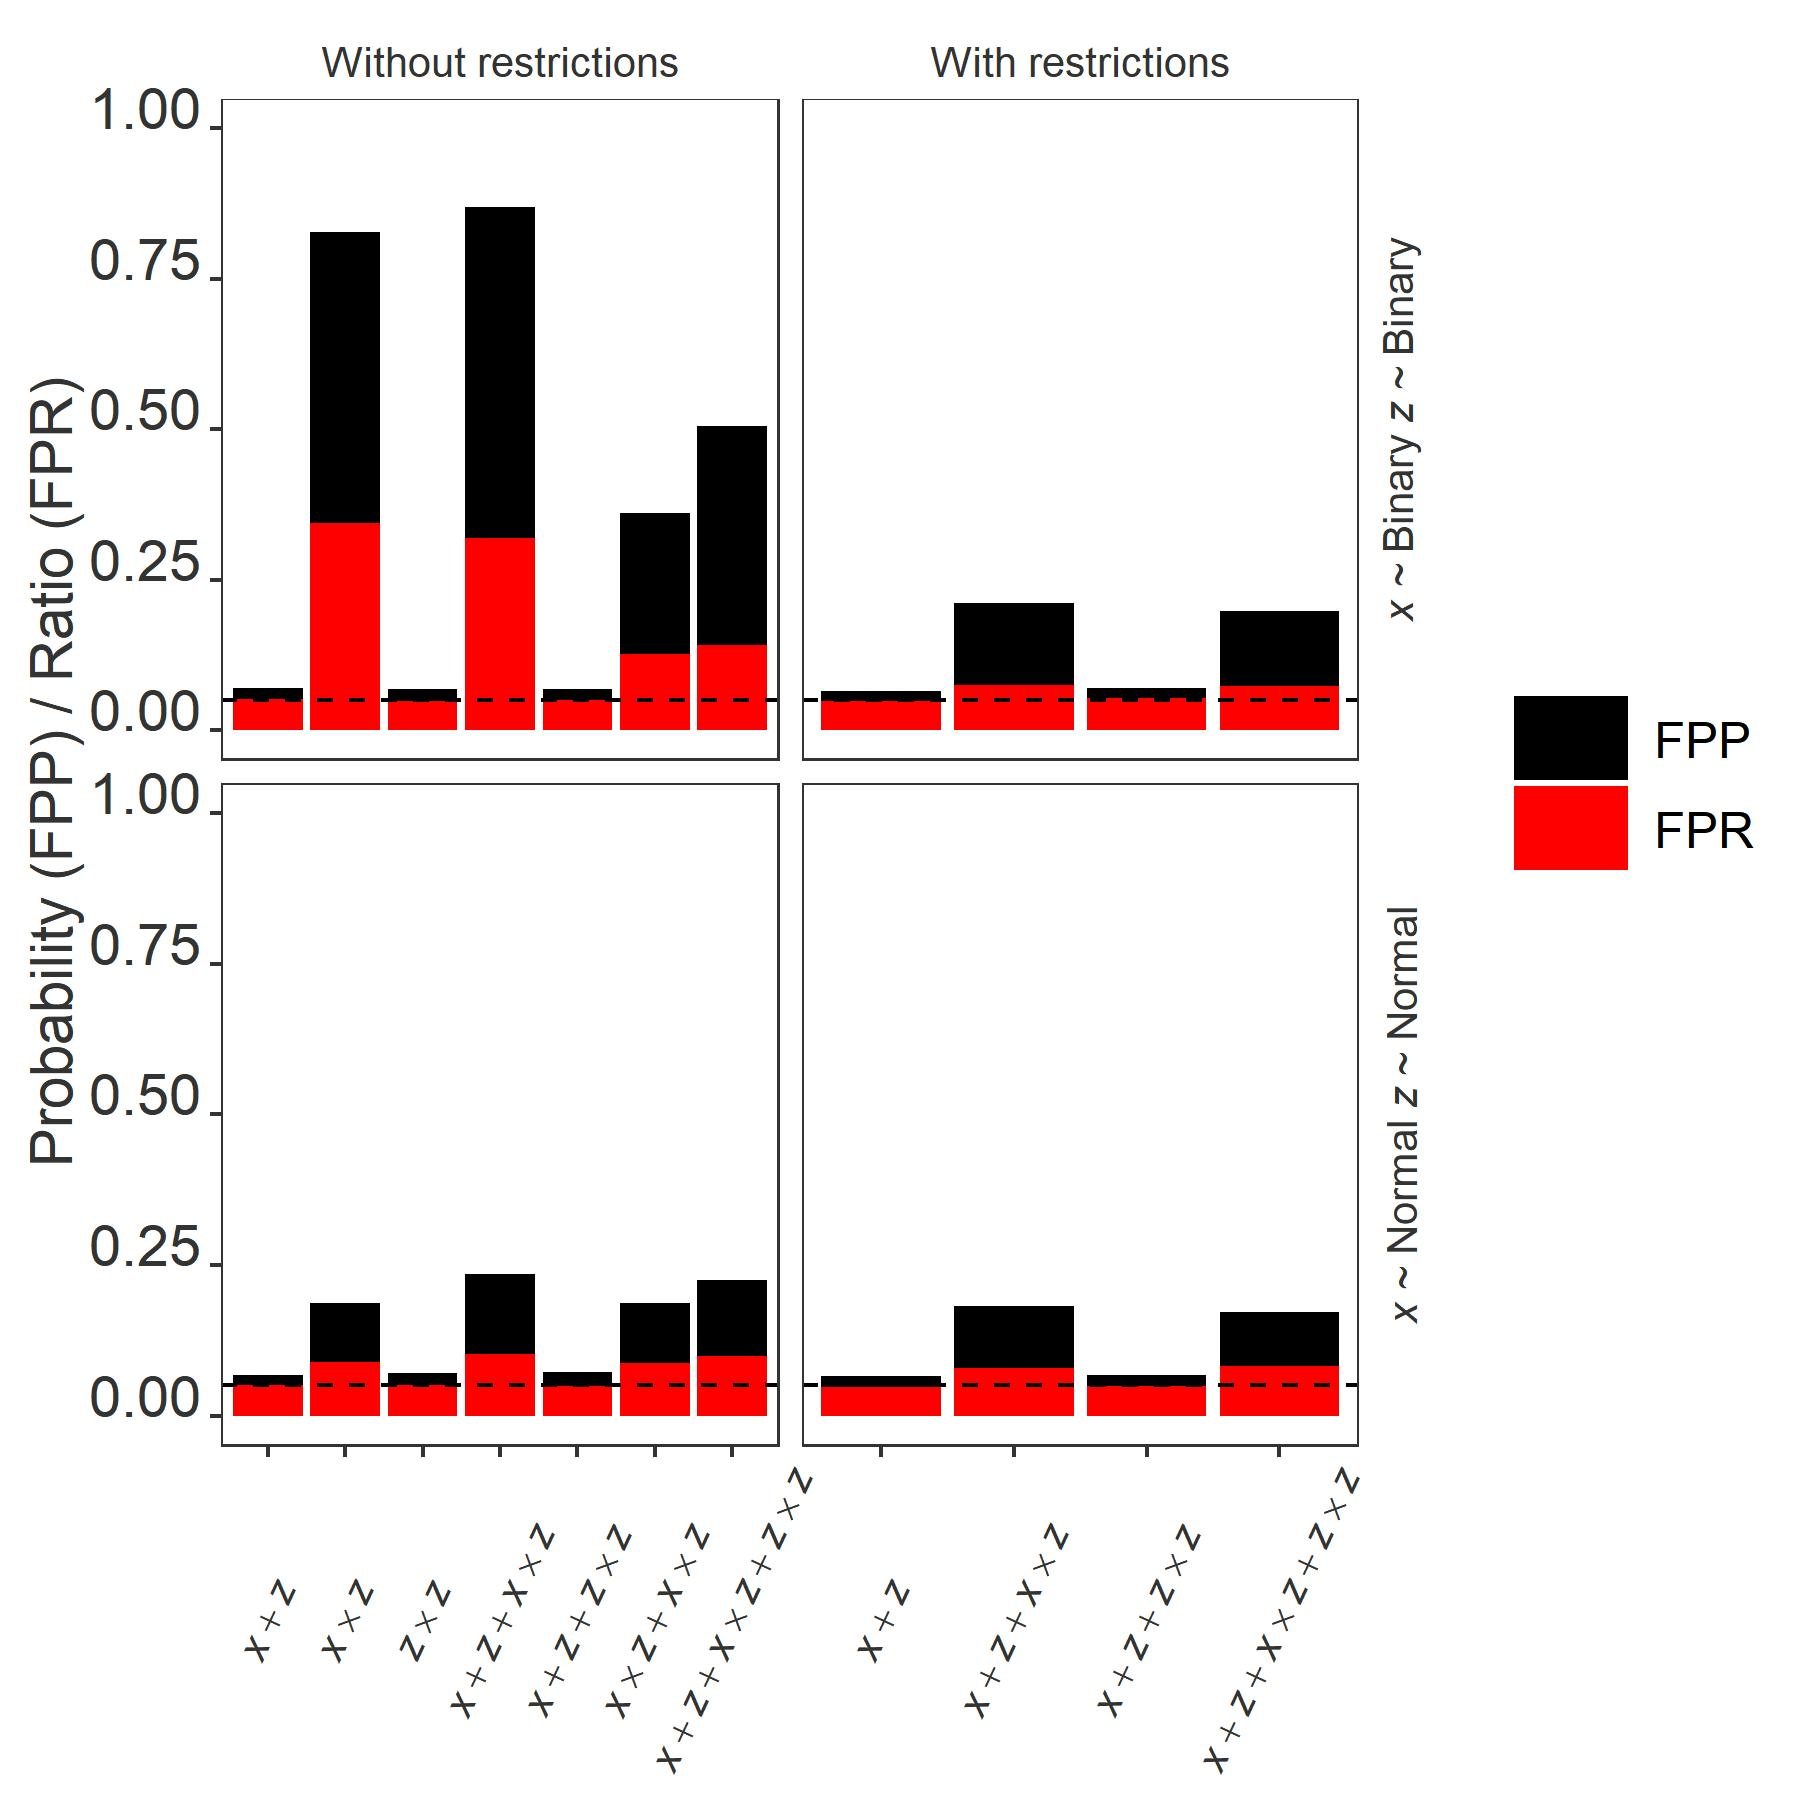
\includegraphics[width=0.6\textwidth]{R/Analysis/Result/Figures/Figure1A.jpeg}
\centering
\caption{The probability of the FPP and FPR given different model sets, the presence of main effects when having interactions and variable of interest distributions. Sample size was set to 200, a correlation between the dependent variable and covariates was \textit{r}=0.2 and we used two covariates. The FPP is shown in black and the FPR in red.}
\label{fig:mainfigure}
\end{figure}

% plot of main analysis
\begin{figure}[hbt!]
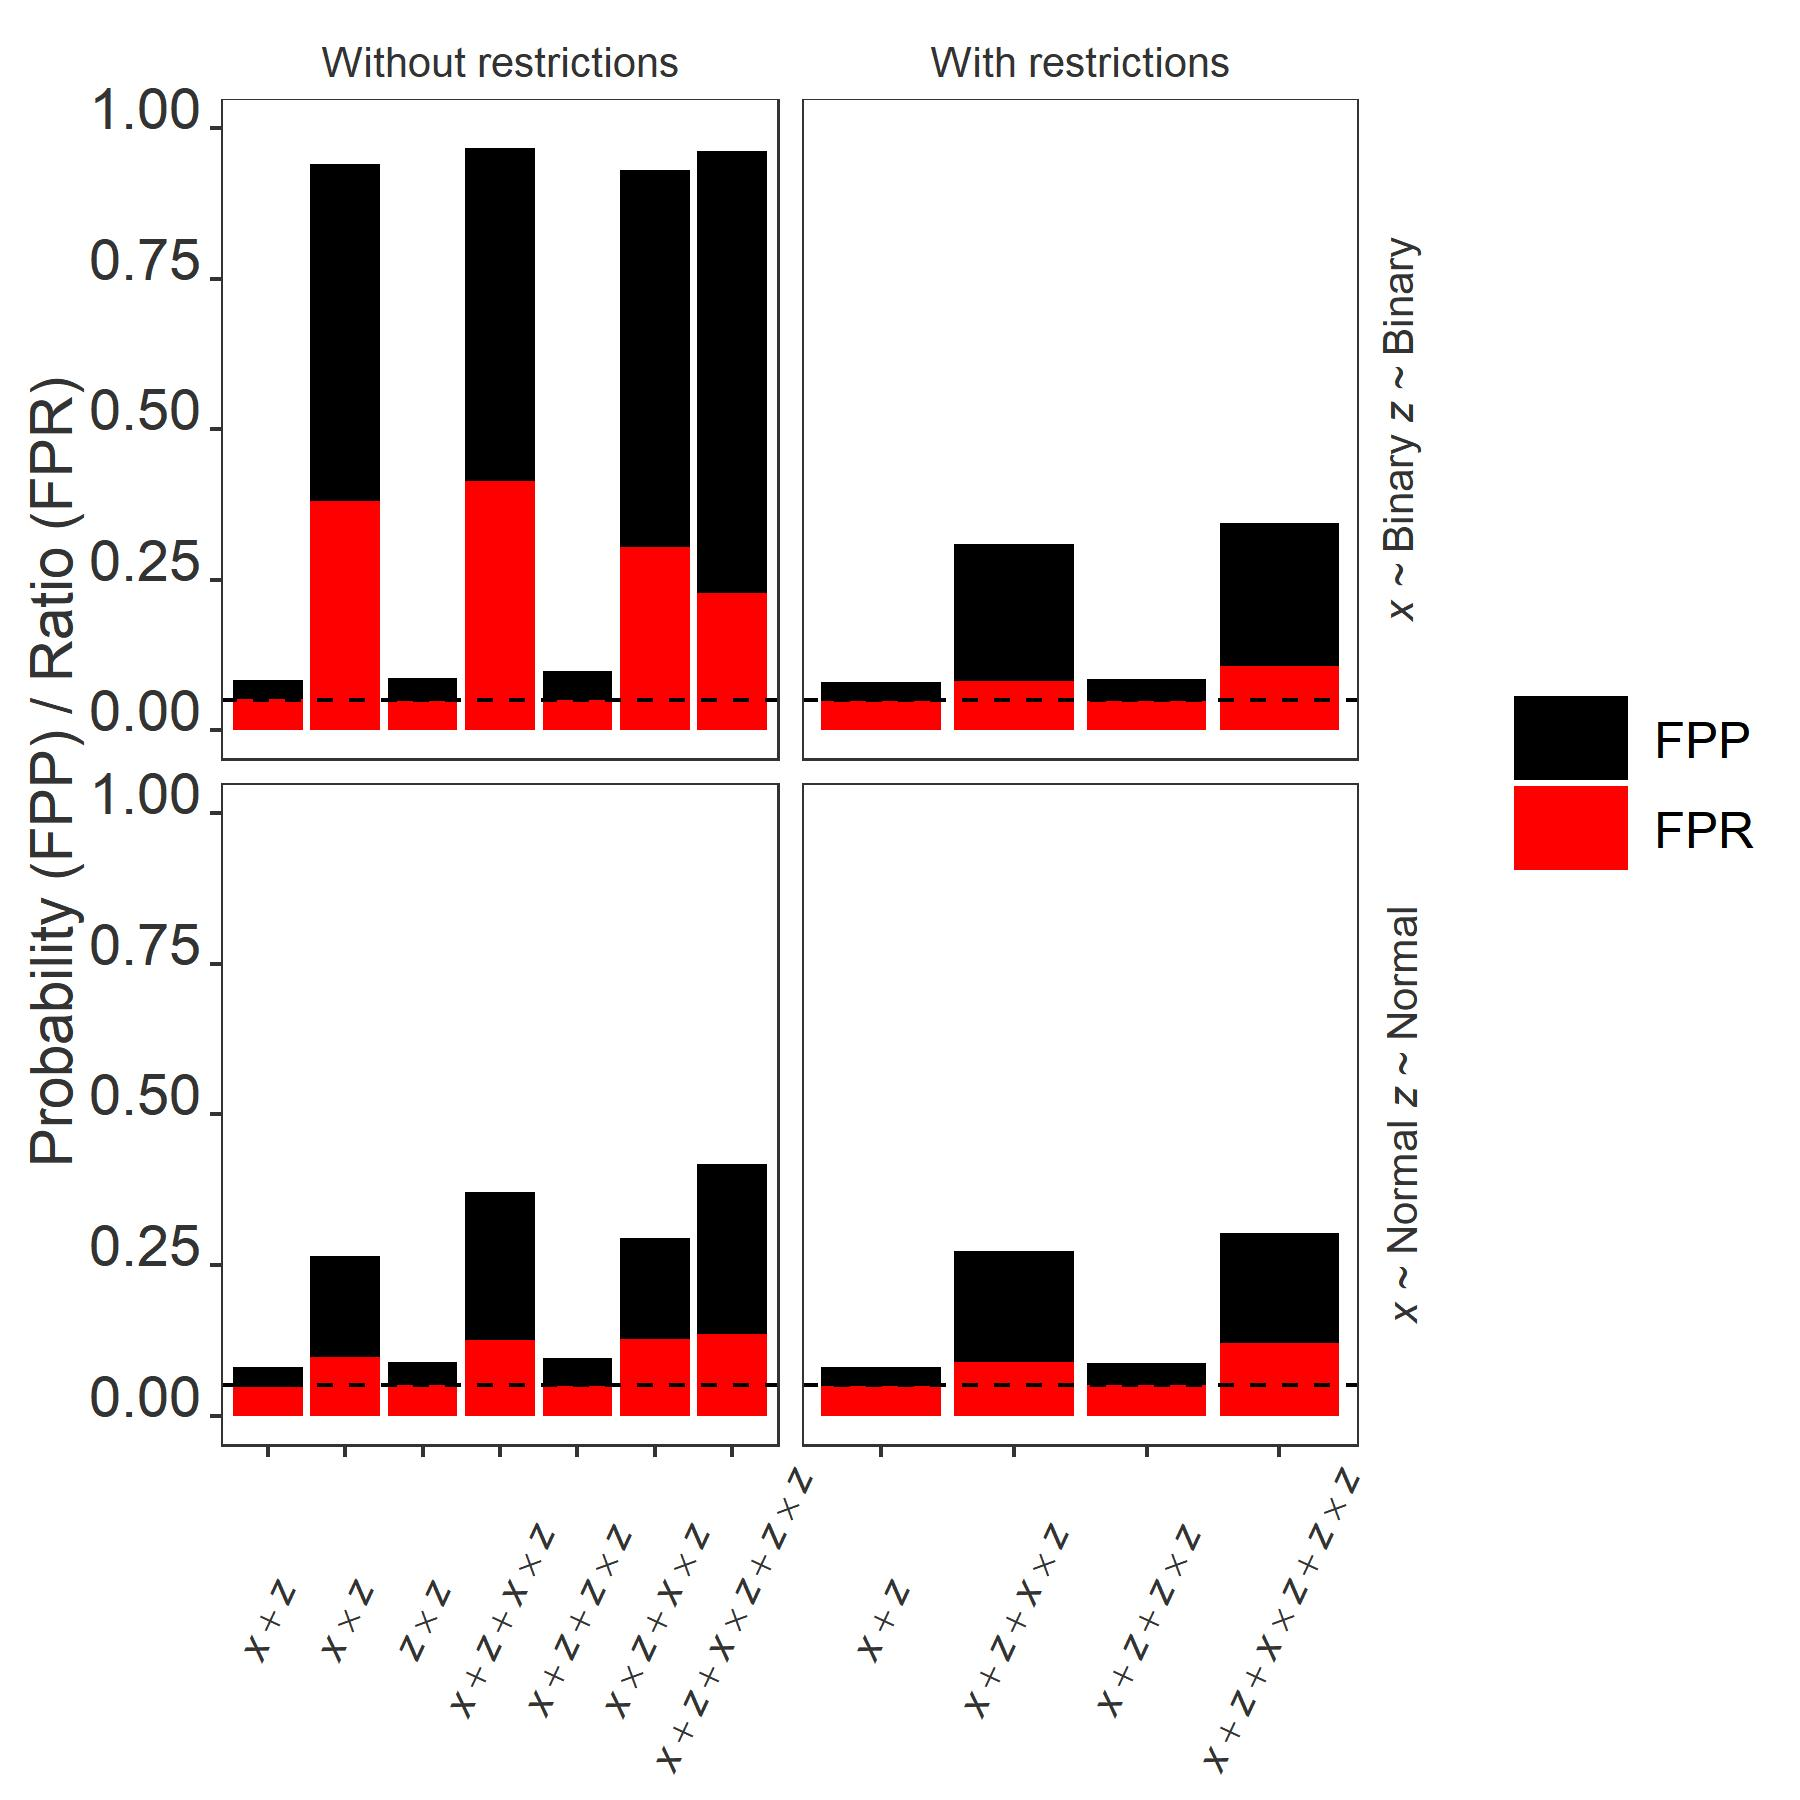
\includegraphics[width=0.6\textwidth]{R/Analysis/Result/Figures/Figure1C.jpeg}
\centering
\caption{Added effect of using one more covariate (three in total) on the FPP and FPR. The description of the figure is otherwise the same as for Figure 1.}
\label{fig:mainfigure}
\end{figure}

\subsection{Outlier criteria}
Here we were interested in how outlier deletion affected the FPP and FPR across the different model sets. Therefore, we plotted the added effect of using the four different outlier criteria compared to not using any such criteria. Again, the sample was set to 200, and all binary variables where dummy coded. Figure 3 shows the added effect of using the outlier criteria. It can be seen that outlier deletion had a different added effect on the different model sets and data structures. The main contribution was within the sets where there were interactions between the covariates. Overall, the added effect to the FPP was between 4\% and 19.4\% for model sets where there was still room for an added effect. The lower added effects seen in some cases came from the fact that the FPP was already close to 100\%. This was the case for the sets where the variables were binary and there was an interaction between the variable of interest and the covariates and where we allowed for models that did not have the main effect present. Using outlier criteria did not increase the FPR and in some cases deleting outliers even decreased the FPR. 

\begin{figure}[hbt!]
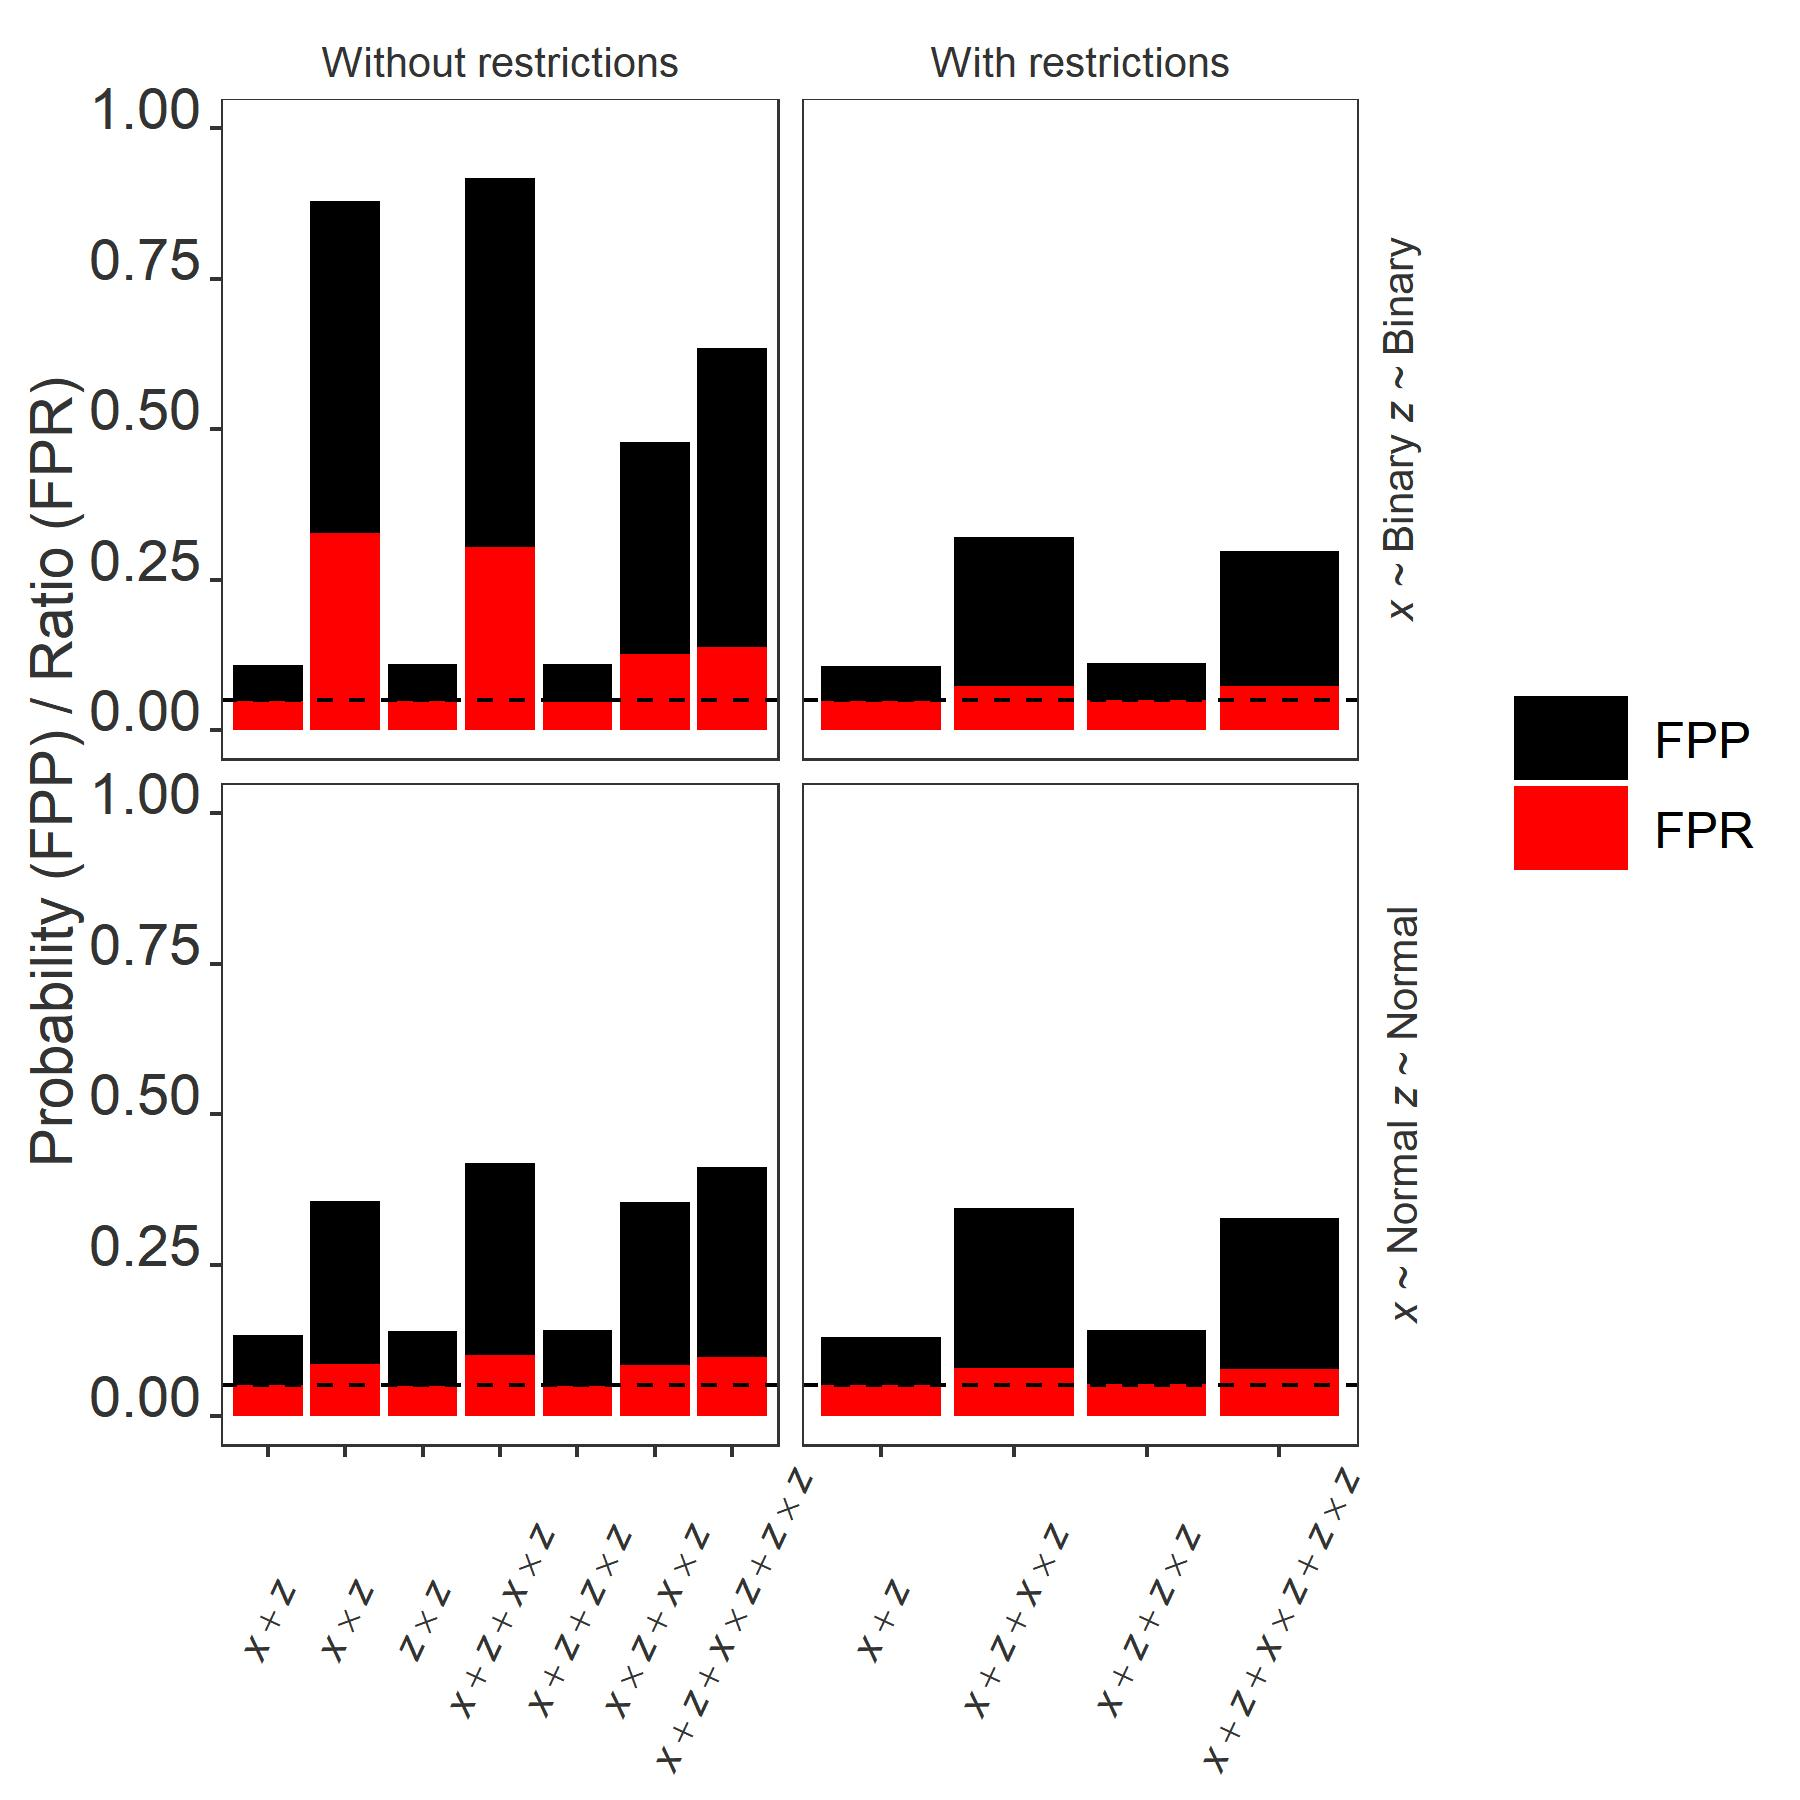
\includegraphics[width=0.6\textwidth]{R/Analysis/Result/Figures/Figure1B.jpeg}
\centering
\caption{Added effect of using multiple outlier criteria. Black denotes the added effect to the FPP and red denotes the added effect to the FPR.  The description of the figure is otherwise the same as for Figure 1.}
\label{fig:mainfigure}
\end{figure}

\subsection{Multiple dependent variables}
Here we looked at the effect of having multiple dependent variables on the FPP and FPR across different sets of the models. We did not specify any outlier criteria and all binary variables were dummy coded. Collecting multiple dependent variables and using their average increased the FPP. This was a general result regardless of data structures, model sets, and whether main effects were included or not. The effect of using two dependent variables and their average can be seen in Figure S3 in supplementary information. This increase was the highest for the sets where there were interactions between the variable of interest and the covariates, no matter the data structure and other specifications. For these sets, the increase in the FPP was around 15\%. The increase in the FPR seems to be mainly driven by the increase in the number of models, as the FPR did not increase for any of the sets. 

\subsection{Sample size}
Increasing the sample size and thereby the precision of the estimates did not seem to lower the FPP. Even worse, when the main effects were not included, the larger sample size increased the FPP when there was interactions between variable of interest and covariate and these were binary (See Figure 4). In this case, the FPP went just under 100\% as the sample size increased to 300. The larger sample did not only increase the FPP, but also the FPR. The FPR got as high as 42\% for the HCI set with binary data and no restrictions. For continues covariates, the results looked the same regardless of main effects following interactions or not, but there was still no decrease in FPP and FPR from increasing the sample size (i.e., the FPP and FPR remained roughly the same for all tested sample sizes). 


\begin{figure}[hbt!]
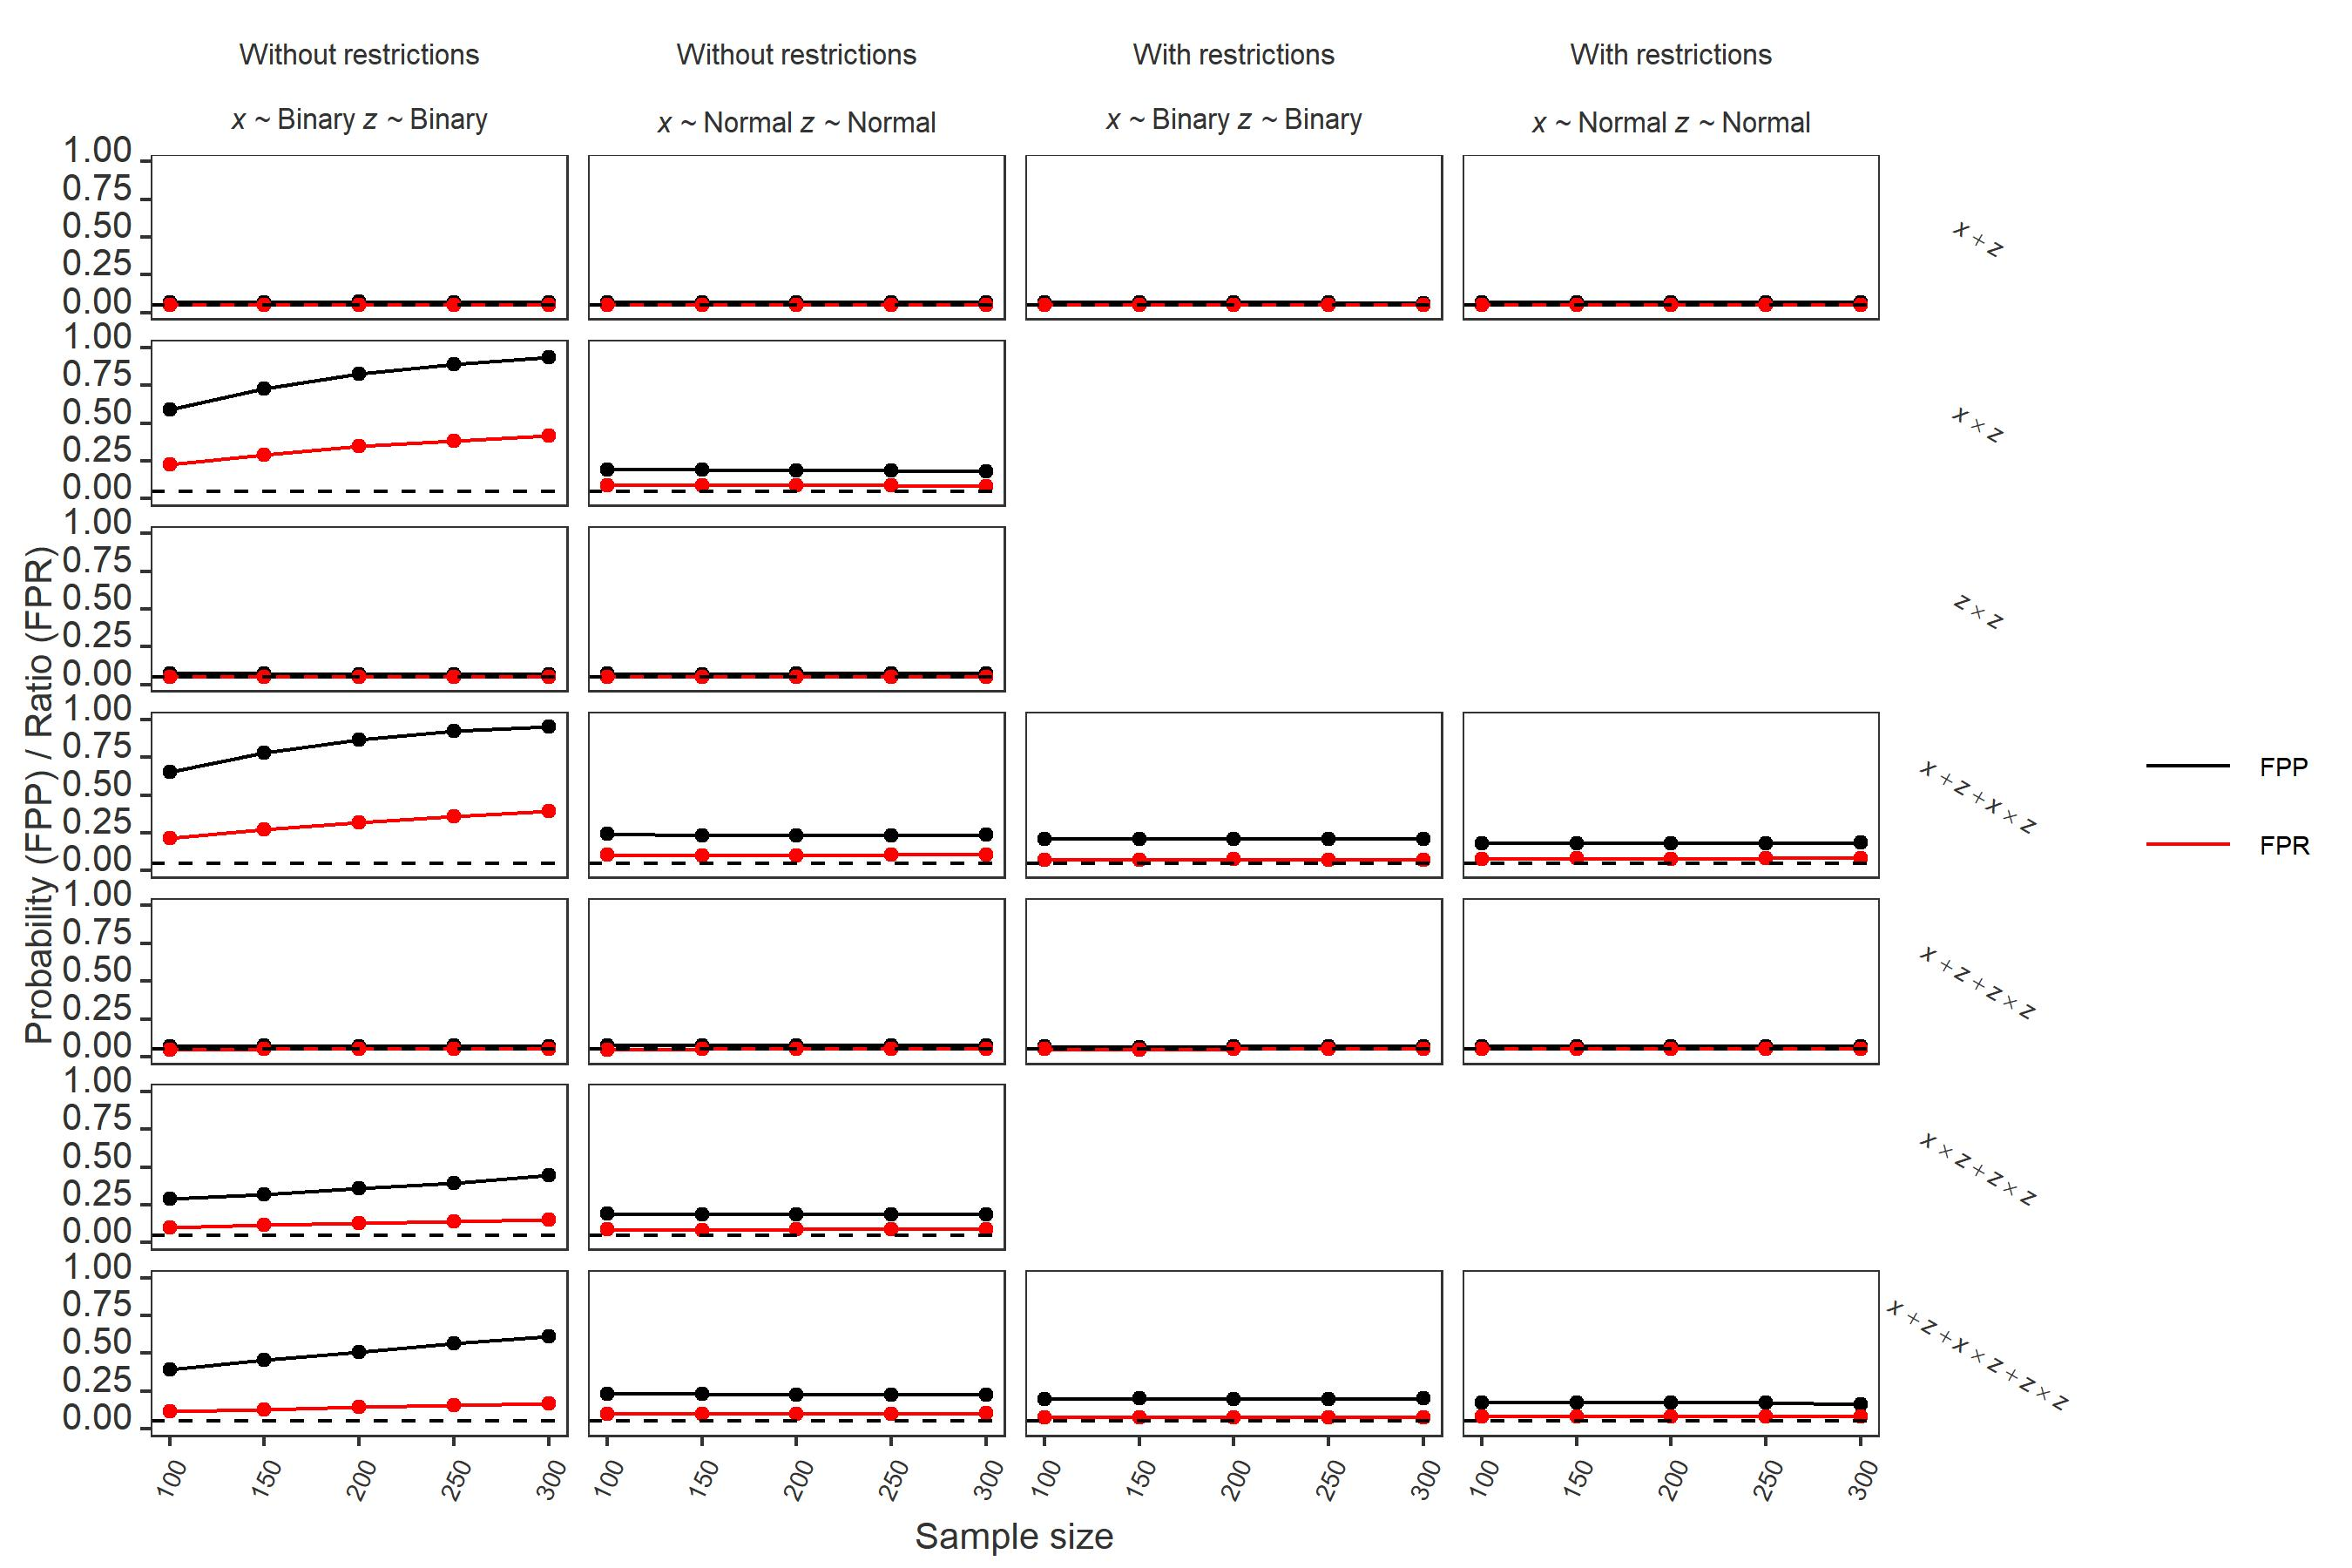
\includegraphics[width=0.9\textwidth]{R/Analysis/Result/Figures/Figure1D.jpeg}
\centering
\caption{The effect of increasing sample size on the FPP and FPR. Black denotes the FPP and red denotes FPR. The description of the figure is otherwise the same as for Figure 1.}
\label{fig:mainfigure}
\end{figure}

\subsection{Correlation}
A higher correlation between the dependent variable and the covariates also increased the FPP and FPR for some model sets. In general, the FPP and FPR were higher as the correlation increased and the main effects did not follow the interactions. The model sets with the highest increase for both the FPP and FPR were the sets that contained HCI. The effect was most pronounced when the variable of interest and covariates were binary (as can be seen in Figure S2). The increase in the FPP for these sets was between 15\% and 23\% when the correlation increased from r=0.2 to r=0.3. When the correlation increased from r=0.3 to r=0.4, the FPP increased only for those sets where there was still room for an increase, since a high number of the sets already had the FPP close to 100\% (see Figure S2). The increase in correlation also affected the FPR for the same sets increasing it to as high as 10\%. When the main effects were present, the FPP and FPR seemed to have a much lower increase (See Figure S2).